\documentclass{article}
\usepackage[utf8]{inputenc}
\usepackage[margin=2cm]{geometry}
\usepackage{natbib}

\title{An agent-based model for city networks based on interactions between firms}

\date{}

\begin{document}

\maketitle

% possible target Journal of Economic Geography? https://academic.oup.com/joeg/
% there is also Economic Geography- % https://www.tandfonline.com/toc/recg20/95/4?nav=tocList
%the editor is Jose Rodriguez-Pose from LSE, I just spoke to him at RSA conf, maybe it will be less econometric than JEG

\section{Introduction}

\citep{taylor2001specification} world city network driven by interactions between firms/behavior of firms
\citep{martinus2018global} combination of different types of proximity in inter-urban firm networks: economic, sociocultural, geopolitical - implies spatial and non-spatial 
\citep{pan2017mapping} different types of linkages: e.g. services here, but not only. All sectors should be taken into account first.

The originality of the present paper is to approach these issues within the system of cities framework \citep{berry1964cities}, where the position and dynamics of cities in the socio-economic world-wide space can be considered by their interactions with other cities \citep{pumain1997pour}. We examine the interactions of european cities within firm linkages. 

\cite{dai2016generative} simpler urban network generative model

\cite{martinus2019brokerage} role of small countries

\cite{dawley2019creating} regional policies for insertion in global network

\cite{turkina2016structure} networks of industrial clusters

\cite{gluckler2016relational} positioning within networks


We compare the model to real data on transnational firm networks defined by ownership links at city-level, by the means of the Bureau Van Dijk's \emph {FAME} database with a graph theory application. 

\section{Model}

\subsection{Rationale}

\begin{itemize}
    \item Single level model: scale of cities - firms induce the links but are not represented in the model
    \item Cities are defined by their profile regarding the proportion of firms in the different sectors
    \item Links between cities are created in an iterative way, with the combination of several drivers:
    \begin{itemize}
        \item geographical proximity (distance or effective accessibility depending on the scale)
        \item geopolitical proximity (belonging to the same ``administrative unit'' $\simeq$ country or single market $\rightarrow$ application to Brexit)
        \item city size (taking not population but an economic variable related to firms avoids adding the dimension of population, simplifies the model) $\rightarrow$ can be combined with geographical distance with a classical interaction model, see \cite{cottineau2015growing}, \cite{raimbault2018indirect}, \cite{favaro2011gibrat}
        \item economic proximity (e.g. cosine distance between sector proximity as done in \cite{2019arXiv190505106C}
        \item previous linkages (taking into account history of previous firm linkages)
    \end{itemize}
    \item These competing drivers are combined - how ? \textit{Options: (i) multiplicative function to get probabilities; (ii) generalization with a multi-attribute Cobb-Douglas; (iii) multi-objective optimization depending on sectors, using Pareto fronts ? - needs empirical evidence; (iv) copula-based combination as done by \cite{2019arXiv190505106C} - copula parameters are free or estimated from real data ?}
    \item The accumulated effects and therefore path-dependency are taken into account into this dynamical model
\end{itemize}


\subsection{Statistical analysis}

% stats to describe the structure of the database, nb of total links, nodes, missing values? + nb of firms per country,  total turnover generated per country etc..

% TODO stat models justifying processes included:
% - poisson regression if we count a number of links?
% - country couples fixed effect to estimate the country distance matrix (as a function of interaction range ?)
% - multilevel modeling ?
% - distribution and properties (spatial stats ?) of sector distributions and similarities


\subsection{Network analysis}

% - network properties of European network (FUAs) in time -> centralities (! directed links), weighted in/out degree

% - correlation with city size etc (check indics of the simulation model?)

% - correlation FUAs gdp from ucdb / gdp by aggregating firms


\subsection{Model description}

Let $1 \leq i \leq N$ cities defined at time $t$ by their economic structure such that $E_i(t)$ is the total economic volume (GDP) for city $i$ and $S_{ik}(t)$ is a matrix giving economic volume proportions within each economic sector $k$, assuming $K$ economic sectors.

% Q : evolution of volume / populations ? Populations not needed indeed.

The city network evolves at discrete time steps the following way:
\begin{enumerate}
    \item Economic structure of cities are evolved with a city interaction model which can be
    \begin{itemize}
        \item a direct interaction model, according to
        \begin{equation}
            \Delta E_i = g_0\cdot E_i + w_G \cdot \sum_j V_{ij}/<V_{ij}>
        \end{equation}
        \item the Marius model with economic exchanges
    \end{itemize}
    \textit{Baseline: no evolution - on short time spans may be relevant ?}
    \item A new linkage is established
    \begin{itemize}
        \item \textit{rq: as these are done sequentially, it is equivalent to have a fixed time step and a number of linkages per time step, or to do it link by link - in the data-driven version the actual values shall be parametrized, while in the synthetic version this has no importance}
        \item the link is drawn randomly with a probability for it to be $i \rightarrow j$ proportional to a function
    \begin{equation}
        p_{ij} = f(d_{ij},g_{ij},E_i,E_j,s(S_{ik},S_{jk}),w_{ij})
    \end{equation}
    with $d_{ij}$ the geographical distance, $g_{ij}$ the geopolitical/sociocultural distance, $g$ a similarity function between sector structure, $w_{ij}$ the relative size of already existing links.
    \item A simple multiplicative form between the different terms may be too restrictive as it assumes independence between components and an equal share between each. Copula capture a dependency structure but must be parametrized by estimation on real data (\textit{keep it as an option for the data-driven model}). An other option is to use a generalized Cobb-Douglas function \citep{vilcu2011geometric}, where exponents can be kept as free parameters. Furthermore, a natural formulation as a separable gravity model as for cities above is already a particular case of such a function, and taking an exponential gravity potential yields that the decay exponent corresponds to the Cobb-Douglas exponent. We therefore take
    \begin{equation}
     p_{ij} \propto \left(\frac{E_{i}}{E}\right)^{\gamma_F} \cdot \left(\frac{E_{j}}{E}\right)^{\gamma_T} \cdot \left(\frac{w_{ij}}{W}\right)^{\gamma_W} \cdot s(S_{ik},S_{jk})^{\gamma_S} \cdot \exp \left(- \gamma_D \cdot d_{ij}\right) \cdot \exp \left(- \gamma_G \cdot g_{ij}\right)
    \end{equation}
    
    \item Note that: (i) we take an asymmetric influence of sizes, assuming that link directions are important (similarly the similarity function $s$ may be taken as asymmetric); (ii) the influence of previous links is similar to a preferential attachment process; (iii) we do not renormalize the exponents to 1 (which is different than renormalizing the probability), to ensure to include convex functions.
    \item We take for the sake of simplicity (\textit{should be amended/validated/tested with an asymmetric function in a further version}) we take a cosine similarity between the sector structures, given with such probability vectors (size effect is already taken into account) by
    \begin{equation}
        s\left(S_{ik},S_{jk}\right) = \sum_{k=1}^{K} S_{ik} S_{jk}
    \end{equation}
    
    \item The ``geopolitical/sociocultural'' distance remains abstract and should be parametrized (see setup below) and estimated in the data-driven setting.
    \item %\textcolor{red}
    TODO the path dependency $w_{ij}$ could (or should ?) be decomposed into in/out degree for origin and destination ? (then stronger self-reinforcment effect)
    \end{itemize}
\end{enumerate}

\subsection{Model setup}

\subsubsection{Synthetic setup}

Let consider the simplest synthetic setup possible:
\begin{itemize}
    \item cities are distributed randomly in a uniform and isotropic space. The total width of the space $d_{max}$ fixed to 3000km to be approximatively the size of Europe. The number of cities is fixed as $N=700$ to similarly match the European urban system structure (GHS database \citep{Florczyk2019ghs}).
    \item city sizes are attributed with a scaling law (equivalent to have a Zipf law for population and a scaling law for economic size), following an exponent $\beta_0$ (fixed at $\beta_0 = 1.1$ in most experiments when not specified, approximate value for GDP from the GHS database, see \citep{raimbault:halshs-02284897})
    % from the GHS database : scaling GDP - pop ~ 1.1 for Europe, rank size 0.94 -> 1.034 : take 1.1 to simplify - can be paramterized ?
    \item country boundaries are constructed to obtain an approximately equal coverage of the space for a fixed number of countries, what remains consistent with non-correlated city sizes at the scale of the countries as our cities are randomly distributed in space \citep{simini2019testing} (\textit{Note: on this point this may be realistic if staying at a continental level, although we should include realistic size of countries; this paper is surely wrong when changing the dataset used and the scale of analysis, working at the scale of Mega-city regions e.g.}). Therefore, we do a basic spatial k-means clustering with $C = 20$ countries and attribute the country accordingly.
    \item firm sector structure: 
    \begin{itemize}
        \item random probabilities
        \item uniform: then the term of proximity is cancelled, no interest
        \item function of size: larger cities are more diverse, larger cities have more knowledge-based sectors. Test 1: log-normal with slightly increasing width and shifting mode.
        % mode of log normal is exp(mu - sigma ^ 2) ; variance is [exp(sigma^2) - 1]*exp(2 mu + sigma ^ 2)
        % when the pdf is 1 / (x sigma sqrt(2 pi)) * exp (- (ln x - mu) ^ 2 / 2 sigma^2 )
        % -> for largest city stddev = sqrt(variance) = fields / 2 ; for smallest sigma = 1 / nfields
        %  ==> solving for mu and sigma with linear mode and variance as a function of log(E_i)
        % => sigma^2 is the unique positive root of f(X)=0 with f(X) = -3X - 2 ln(exp(X)-1) - ln(e_i)
        % => mu = sigma^2 + ln(e_i)
        %    ~ somehow dirty and not sure that most of the distrib for highest values is within [0,1]
    \end{itemize}
\end{itemize}

! links depend on the sectors: cobb douglas for sector proximity should depend on sector composition ? or several functions ?


\subsubsection{Real data setup}

Data sources:
\begin{itemize}
	\item AMADEUS database for company links
	\item GHS UCDB for GDP of urban built-up areas
	\item Functional urban areas (JRC-EC) for consistent ontology and spatial join between the different sources
	\item Cities GDP can also be computed by aggregating company data: correlation between this approach and the GHS one must be checked
\end{itemize}

If the links are ``complete'' within Europe, the model (i) can be initialized at $t_0$ with the network corresponding to the first date in the dataset; (ii) adjustment error is computed on the later dates.

%%%
% with new dataset we do not have a subsample of companies within a specific country anymore
%More probably, we may have to work on an extract of the AMADEUS database including only links from and to UK-based companies. This constraints imposes modifications on the level to remain consistent:
%\begin{itemize}
%    \item the adjustment error can only be partial and computed on the UK links only
%    \item an initialization method for the missing links must be implemented (e.g. through a statistical analysis? not far from the model then)
%    \item the model can be run without initial links, and an additional parameter sets the duration necessary to reach the time considered as the first date
%\end{itemize}




\subsection{Model indicators}


\subsubsection{Geographical indicators:}

\begin{itemize}
    \item Internationalisation (modularity of countries in the network)
    \item Metropolisation (correlation between weighted degree and city size)
    \item Regionalisation (correlation between length and flow of links, stratified by size of extremities)
    \item Specialisation (correlation between sector proximity and flow of links, stratified by size of extremities)
\end{itemize}


\subsubsection{Network and flows indicators:}

%  networkModularity, networkAvgCommunitySize, networkDegreeHierarchy, networkAvgDegree, networkDegreeEntropy, flowsHierarchy, flowsEntropy, rhoDegreeSize, rhoFlowDistancePos, rhoFlowDistance

\begin{itemize}
    \item Louvain modularity, community sizes
    \item Degree and flows distribution (average, hierarchy, entropy)
    \item Correlations (degree-size, flow-distance)
\end{itemize}

% possible other indics:
% weighted degree distribution (\textit{if it is fat-tailed, log-log power law exponent and adjusted r-squared})
%Sector structure indicators: sector diversity (Herfindhal ?) 





\subsection{Model parameters}

\begin{table}
    \caption{List of parameters, associated processes, and ranges.}
    \begin{center}
    \begin{tabular}{|c|c|c|c|}
    \hline
    Parameter & Name & Process & Range \\\hline
      $\gamma_F$ & Origin &  & $\left[0;10\right]$ \\
    $\gamma_T$ & Destination & & $\left[0;10\right]$ \\
    $\gamma_W$ & Previous links & Self-reinforcement & $\left[0;10\right]$  \\
    $\gamma_D = \frac{1}{d_G}$ & Geographical distance & & $\left[0;10000\right]$ \\
    $\gamma_G  = \frac{1}{d_G}$ & Socio-cultural distance & & $\left[0;10000\right]$ \\\hline
    \end{tabular}
    \end{center}
\end{table}



\section{Results}

\subsection{Implementation}

% Netlogo for vis + scala into spatialdata / urbangrowth ?

% On vine copulas :
%    https://link.springer.com/article/10.1023/A:1016725902970
%    https://www.groups.ma.tum.de/en/statistics/research/vine-copula-models/
%    R package : https://github.com/tnagler/VineCopula
% Q: what would be the meaning on parametrizing interaction function with a real Vine copula? non-linear interactions? (on log, linear combination of factors)

The model is implemented in NetLogo and integrated into the OpenMOLE platform for model exploration \cite{reuillon2013openmole}. NetLogo provides a good compromise between performance and interactive prototyping and exploration.
%We use in particular data structures providing good performances for the type of operations needed (matrices operations for the construction of the utility function e.g.).



%%%%%%%%%%%%%
\begin{figure}
    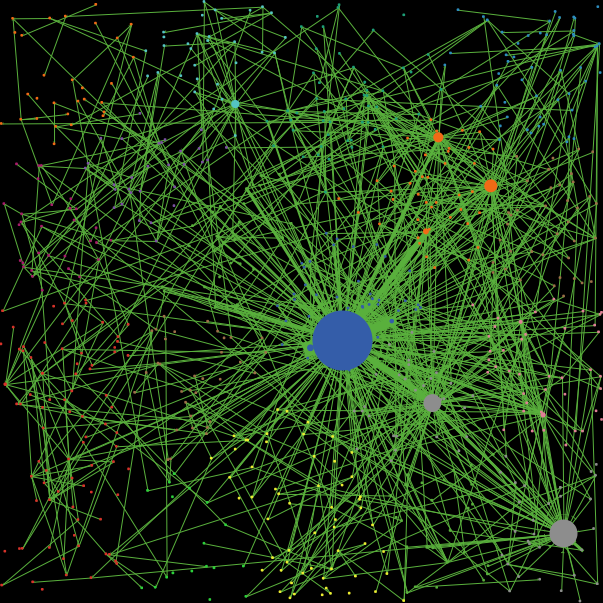
\includegraphics[width=0.48\textwidth]{figures/ex_alleq-highgravity_seed-12102_t1500.png}
    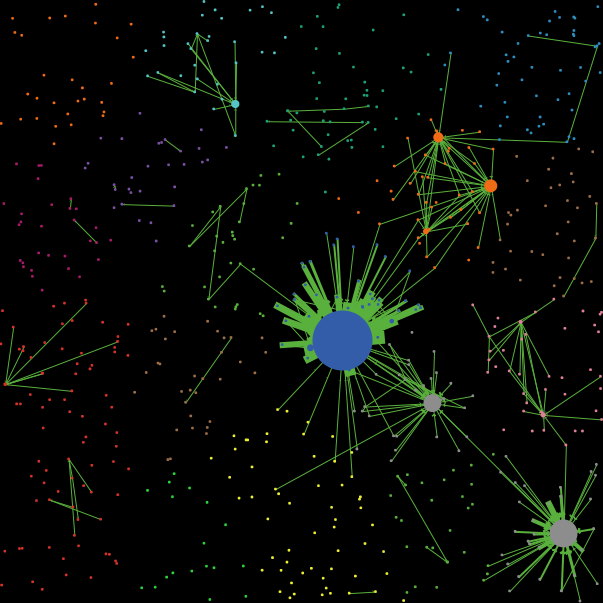
\includegraphics[width=0.48\textwidth]{figures/ex_alleq-lowgravity_seed-12102_t1500.png}	
    \caption{Example of simulated networks at $t=1500$, with a high (resp. low) gravity decay parameter on the left (resp. right).\label{fig:example}}
\end{figure}
%%%%%%%%%%%%%



\cite{railsback2017improving} netlogo perfs 

\subsection{Synthetic city systems}

\subsubsection{Sensitivity analysis and grid exploration}

\paragraph{One factor sampling}
% 20190924_162740_ONEFACTOR_REPLICATIONS_SYNTHETIC_GRID


\begin{figure}
	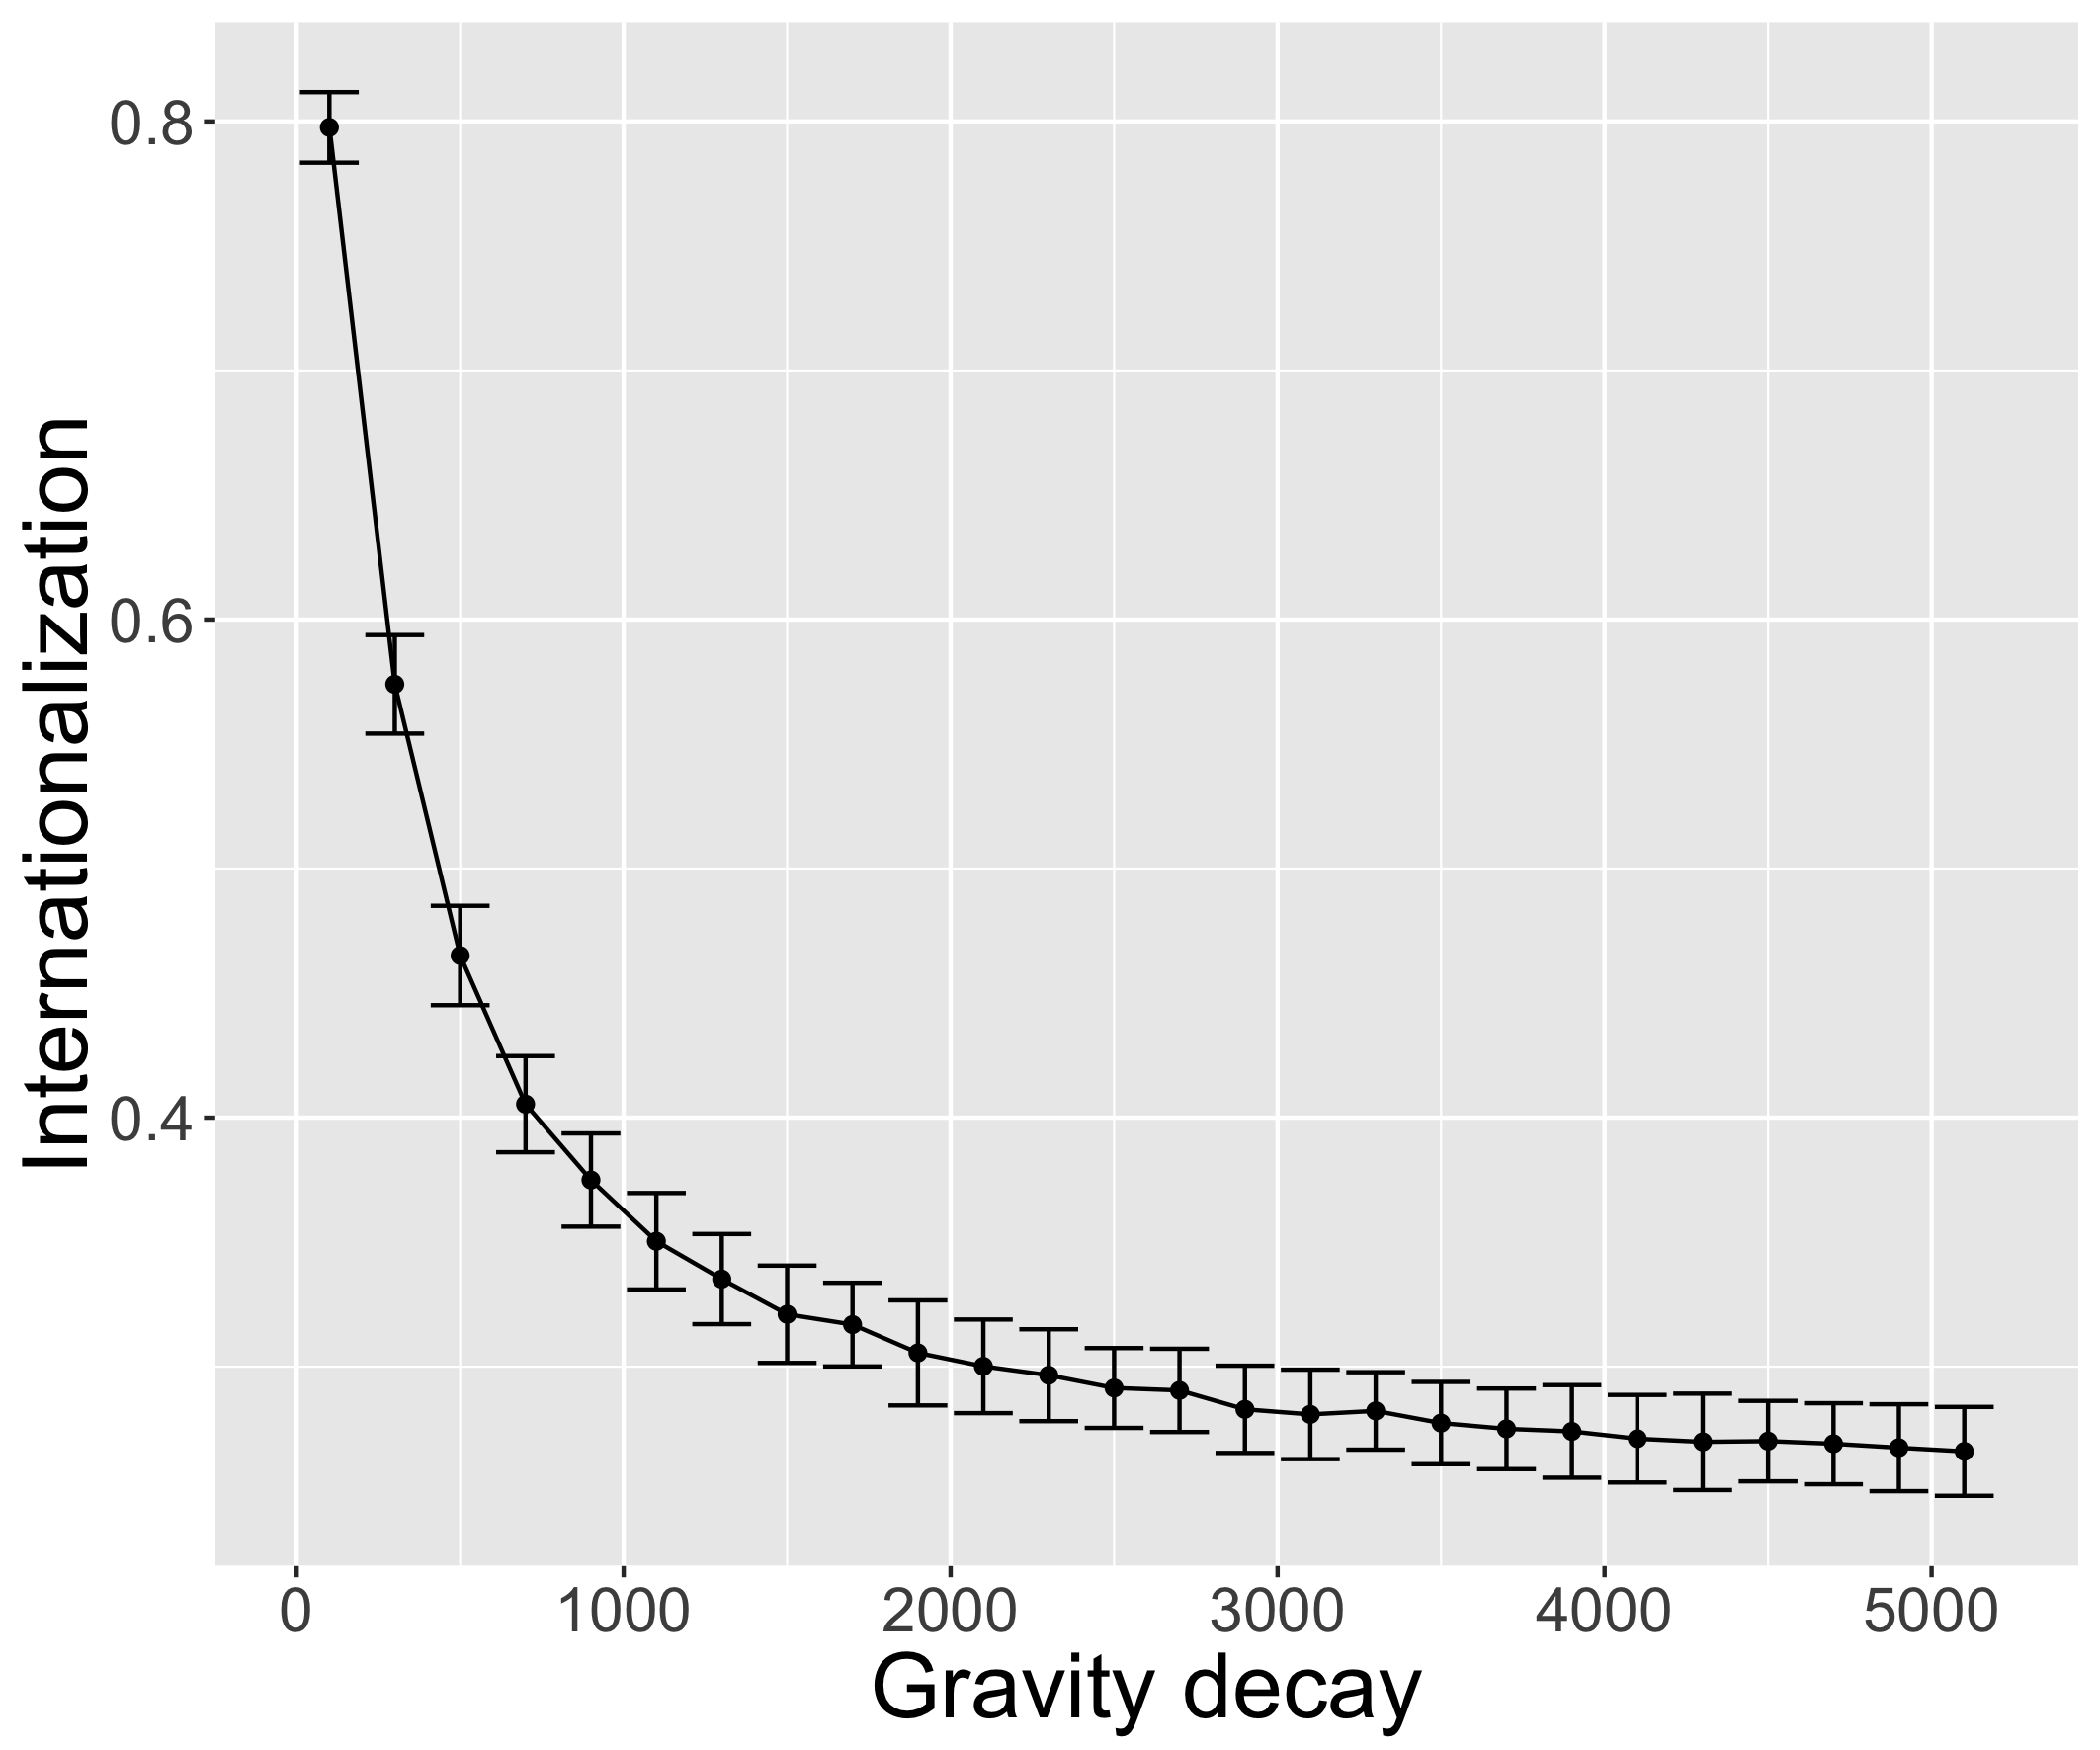
\includegraphics[width=0.48\textwidth]{figures/internationalization-gravityDecay_errorbars.png}
    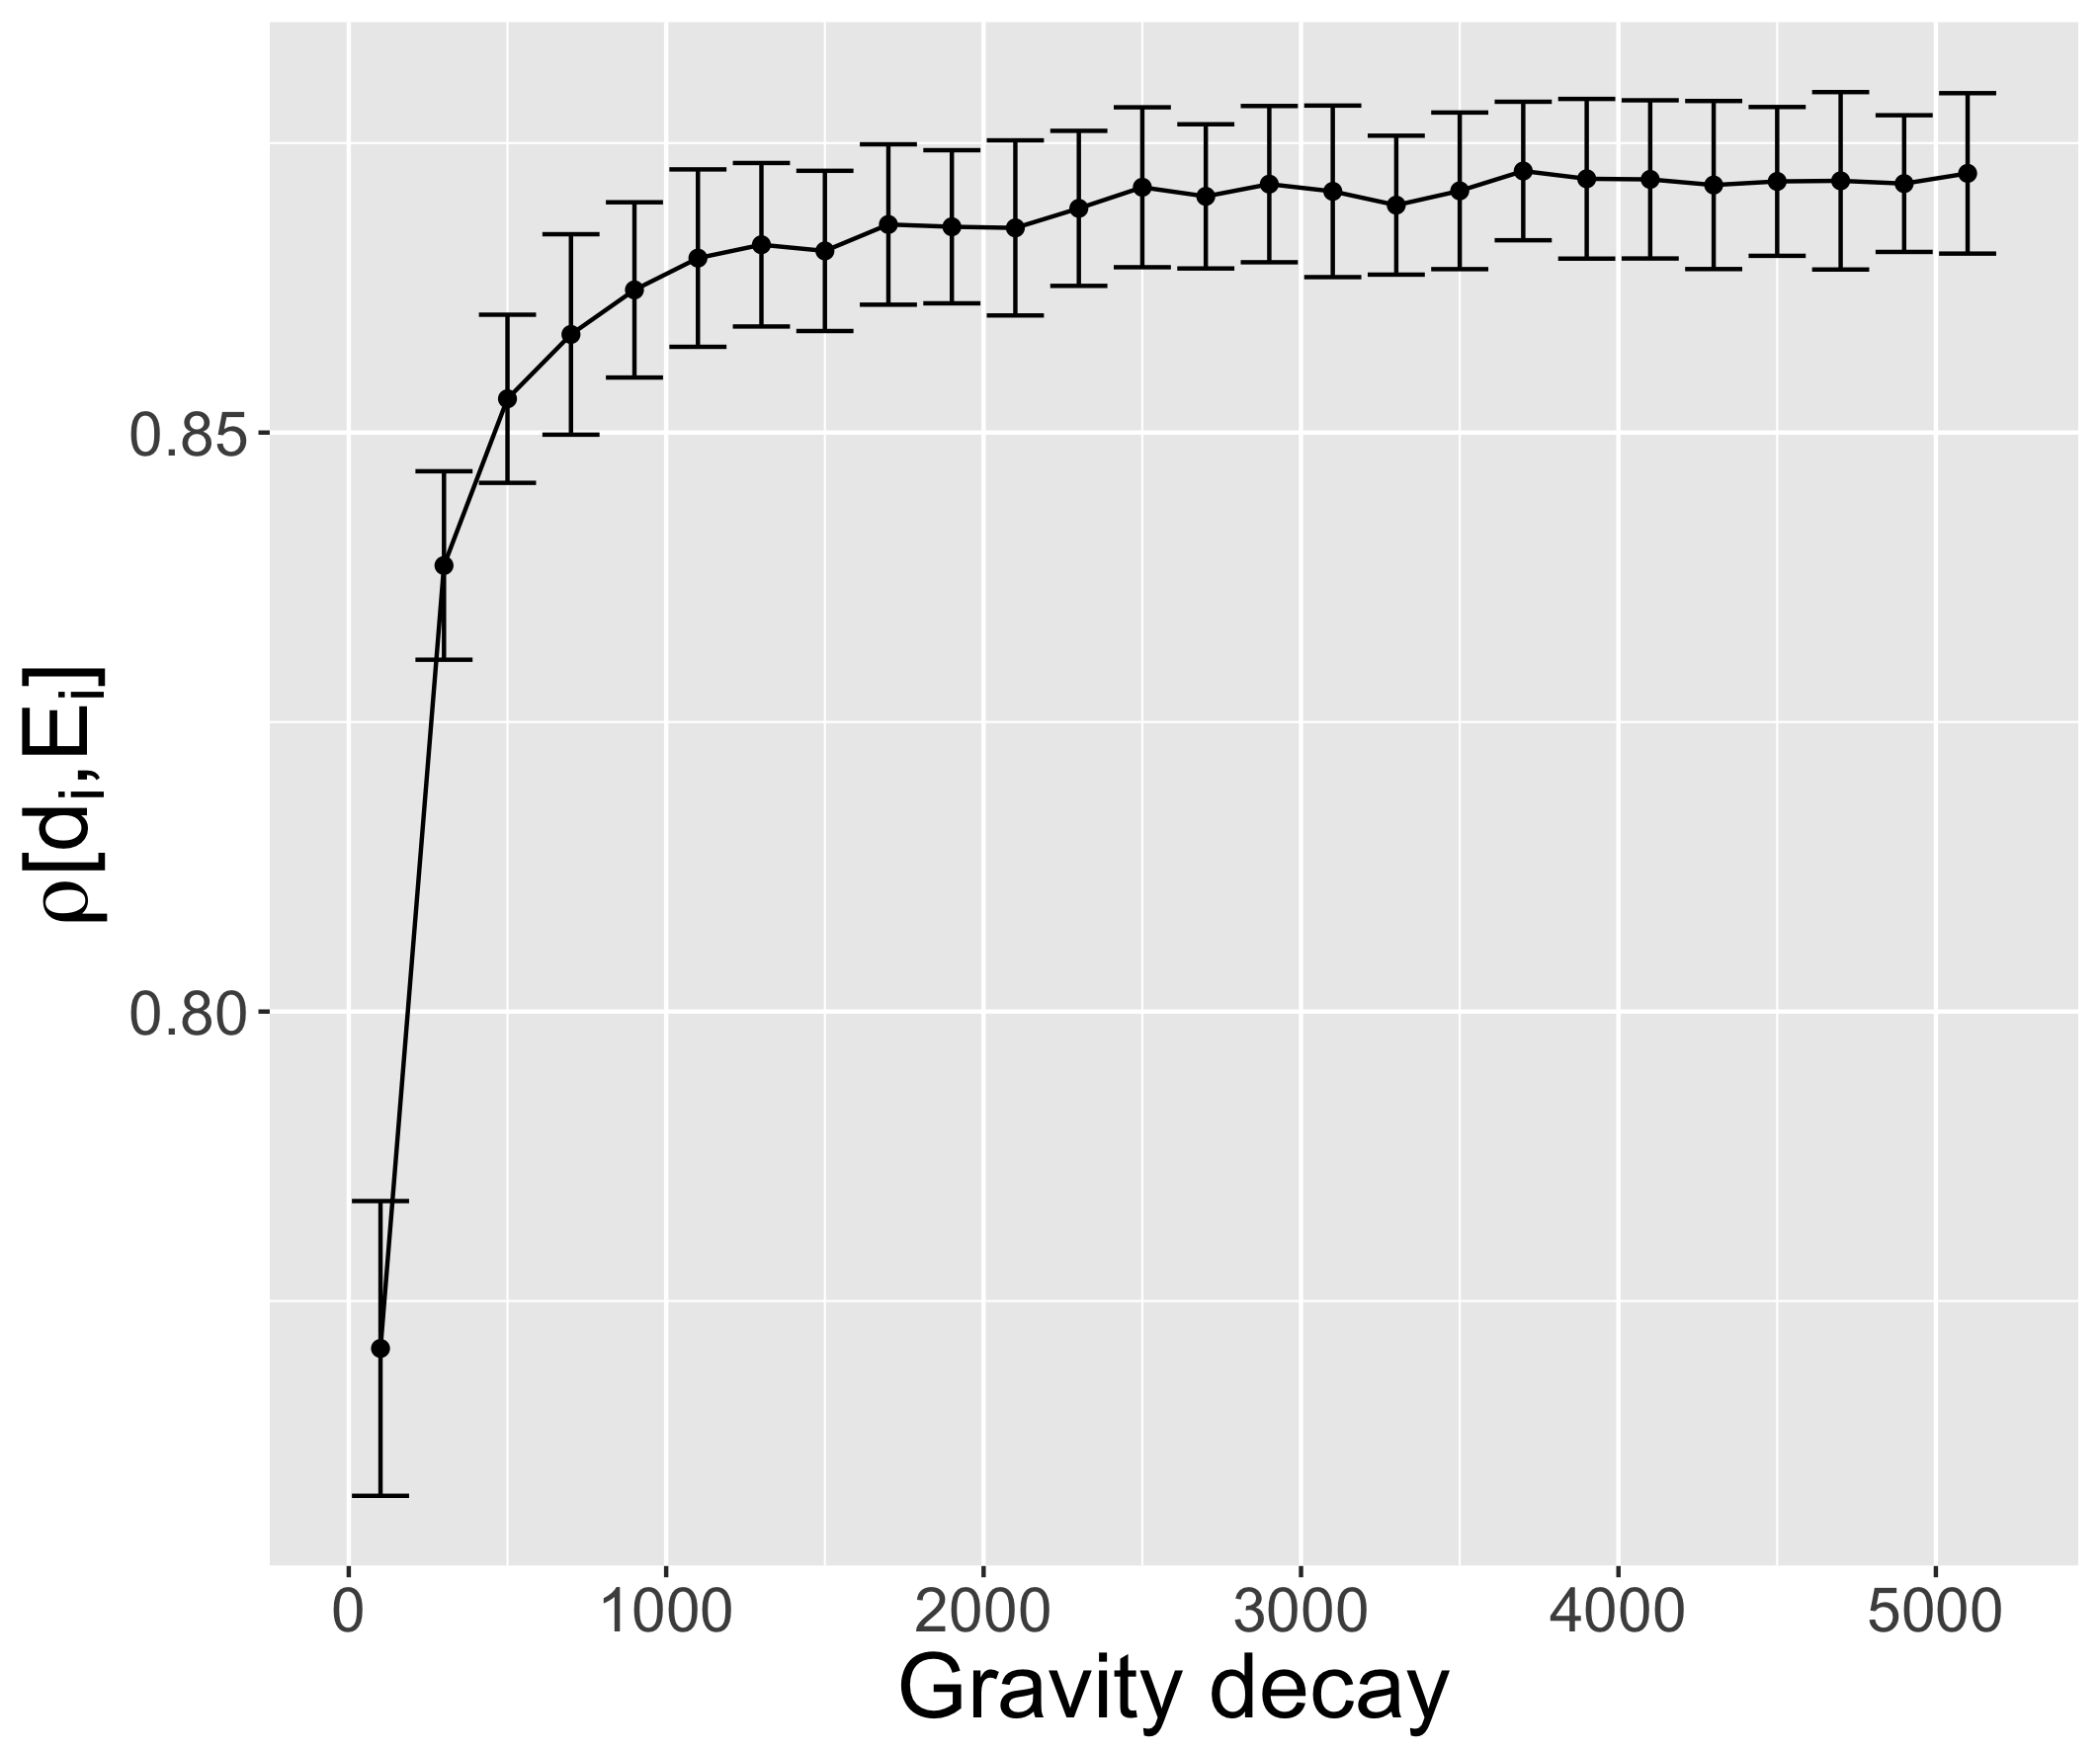
\includegraphics[width=0.48\textwidth]{figures/rhoDegreeSize-gravityDecay_errorbars.png}
    \caption{(Left) Internationalization index decreases exponentially with gravity decay; (Right) Correlation between city weighted degree and size. Both plots show a transition from a local to a global regime.}
\end{figure}



\begin{figure}
    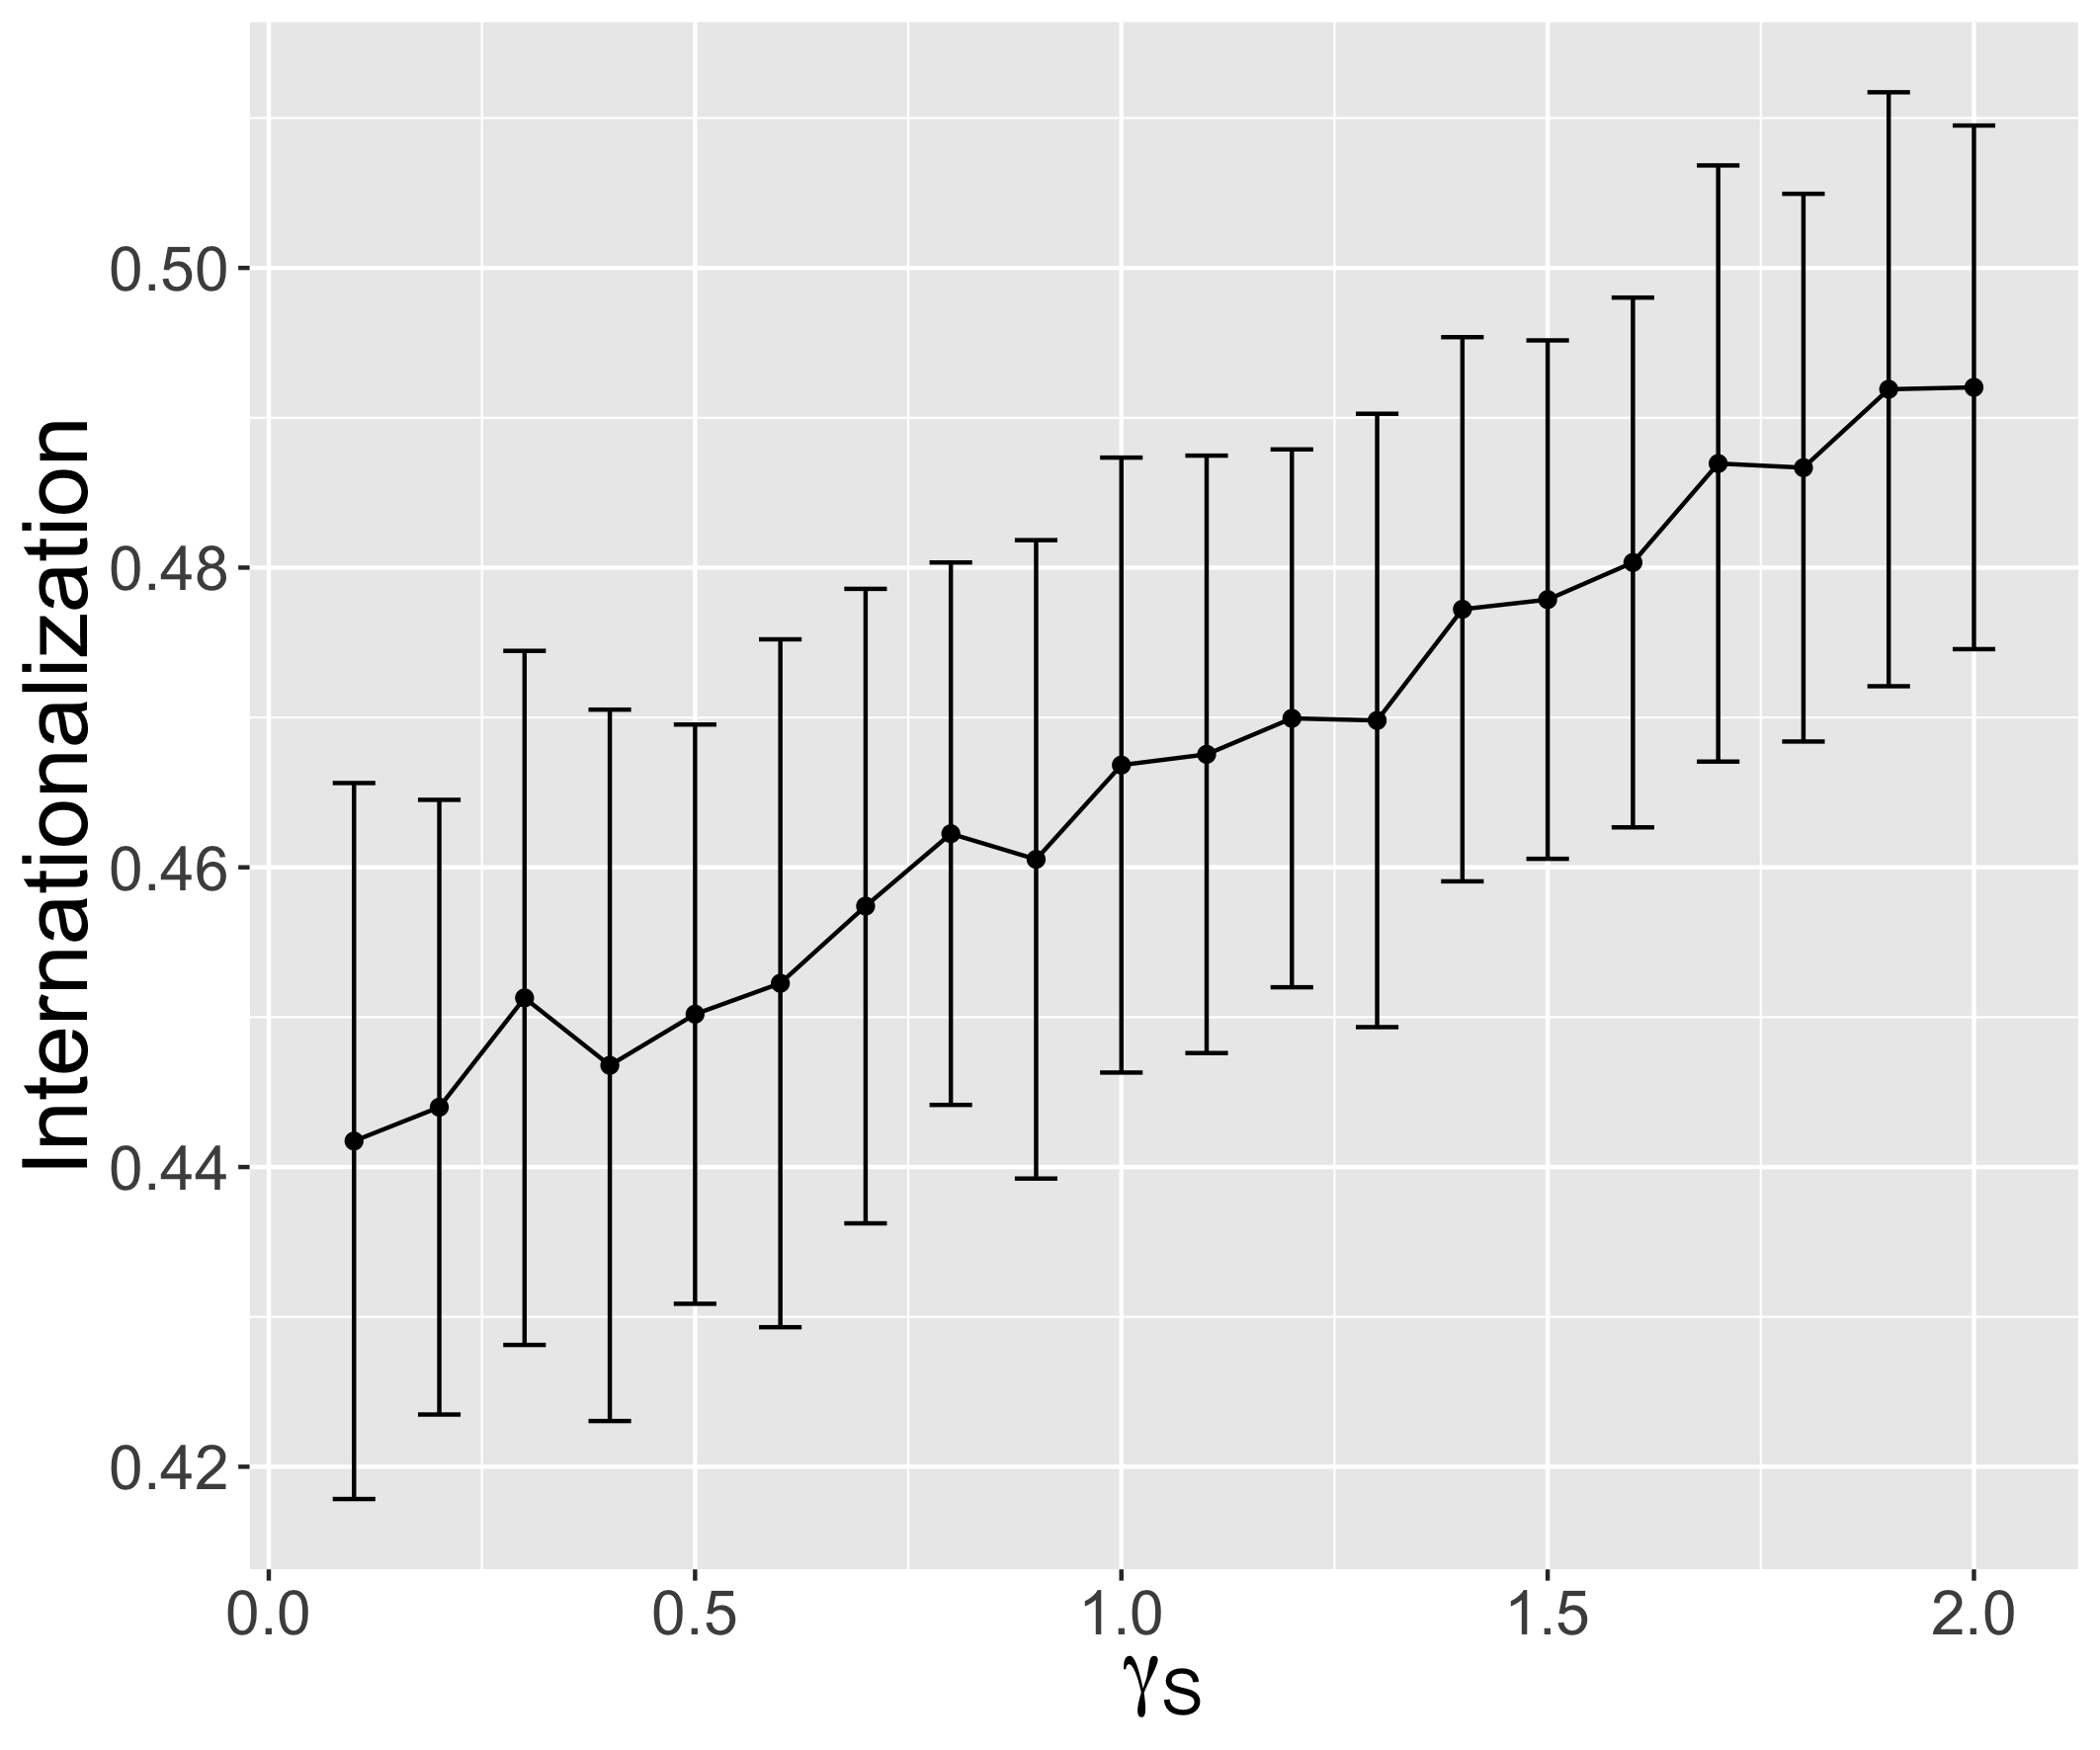
\includegraphics[width=0.48\textwidth]{figures/internationalization-gammaSectors_errorbars.png}
    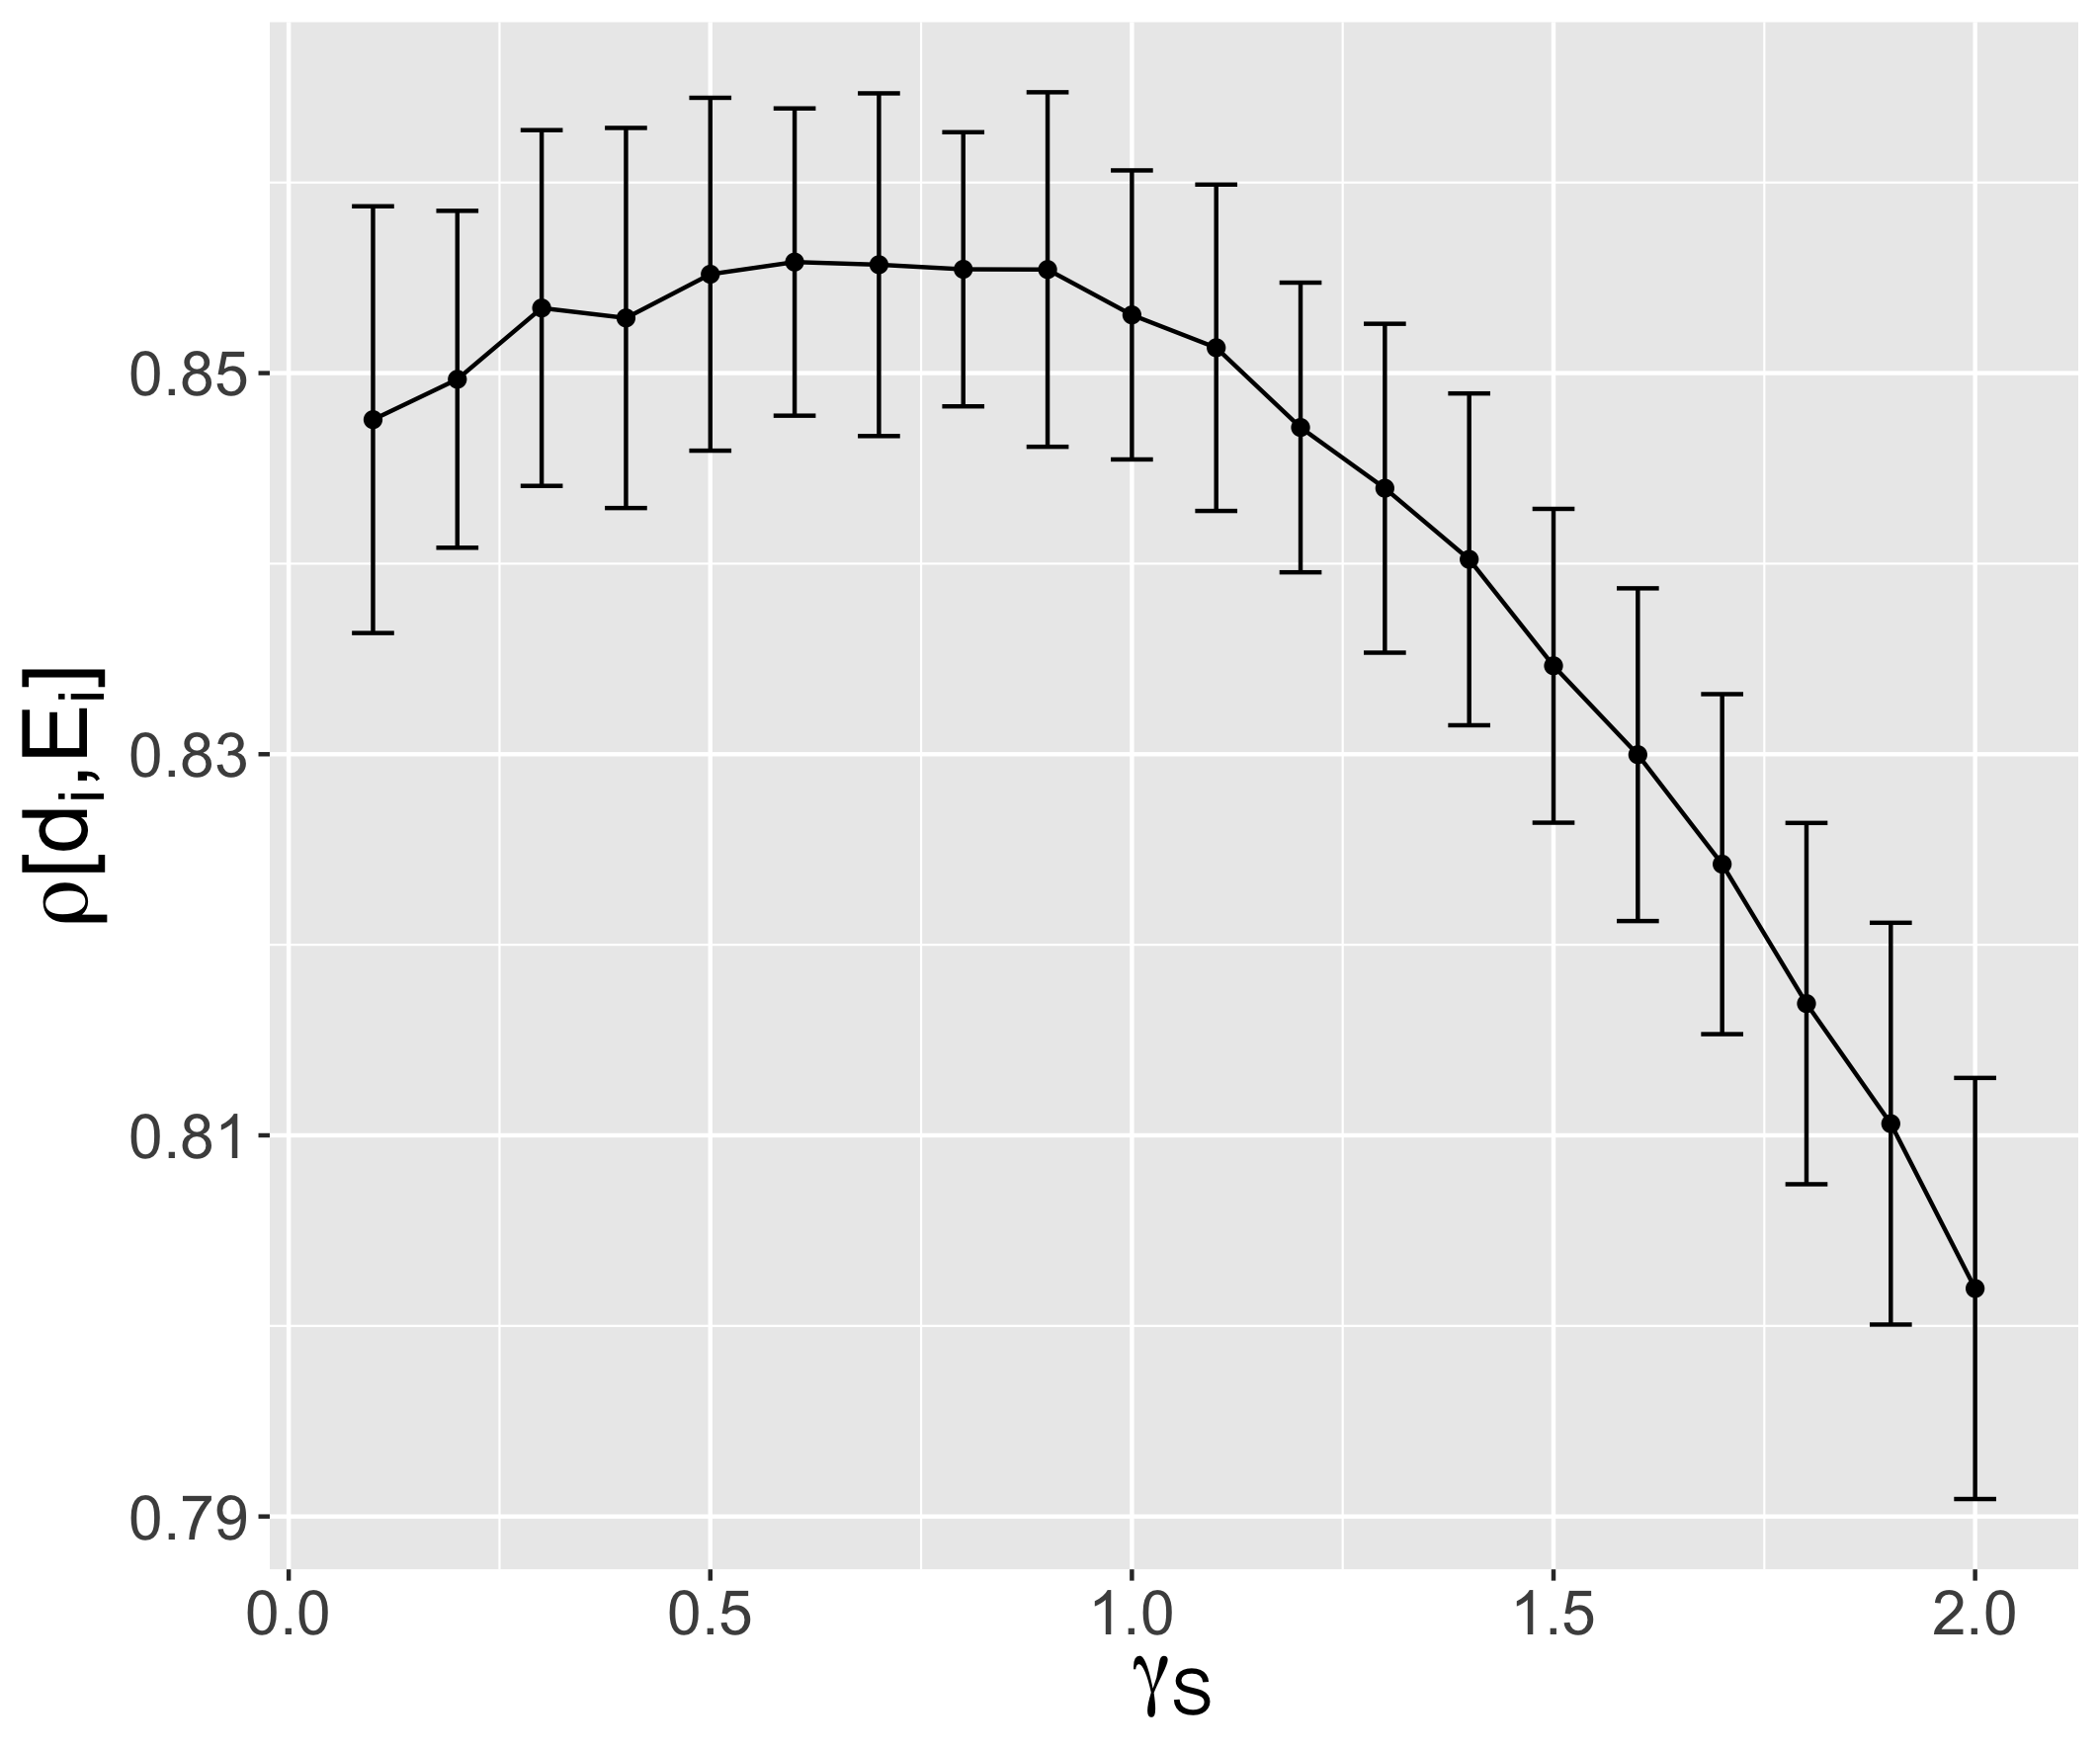
\includegraphics[width=0.48\textwidth]{figures/rhoDegreeSize-gammaSectors_errorbars.png}
    \caption{(Left) Internationalization varies linearly with sector proximity $\gamma_S$; (Right) Correlation between degree and size exhibits a maximum, witnessing an intermediate regime where size is the most important}
\end{figure}


\paragraph{Grid exploration}

\begin{figure}
    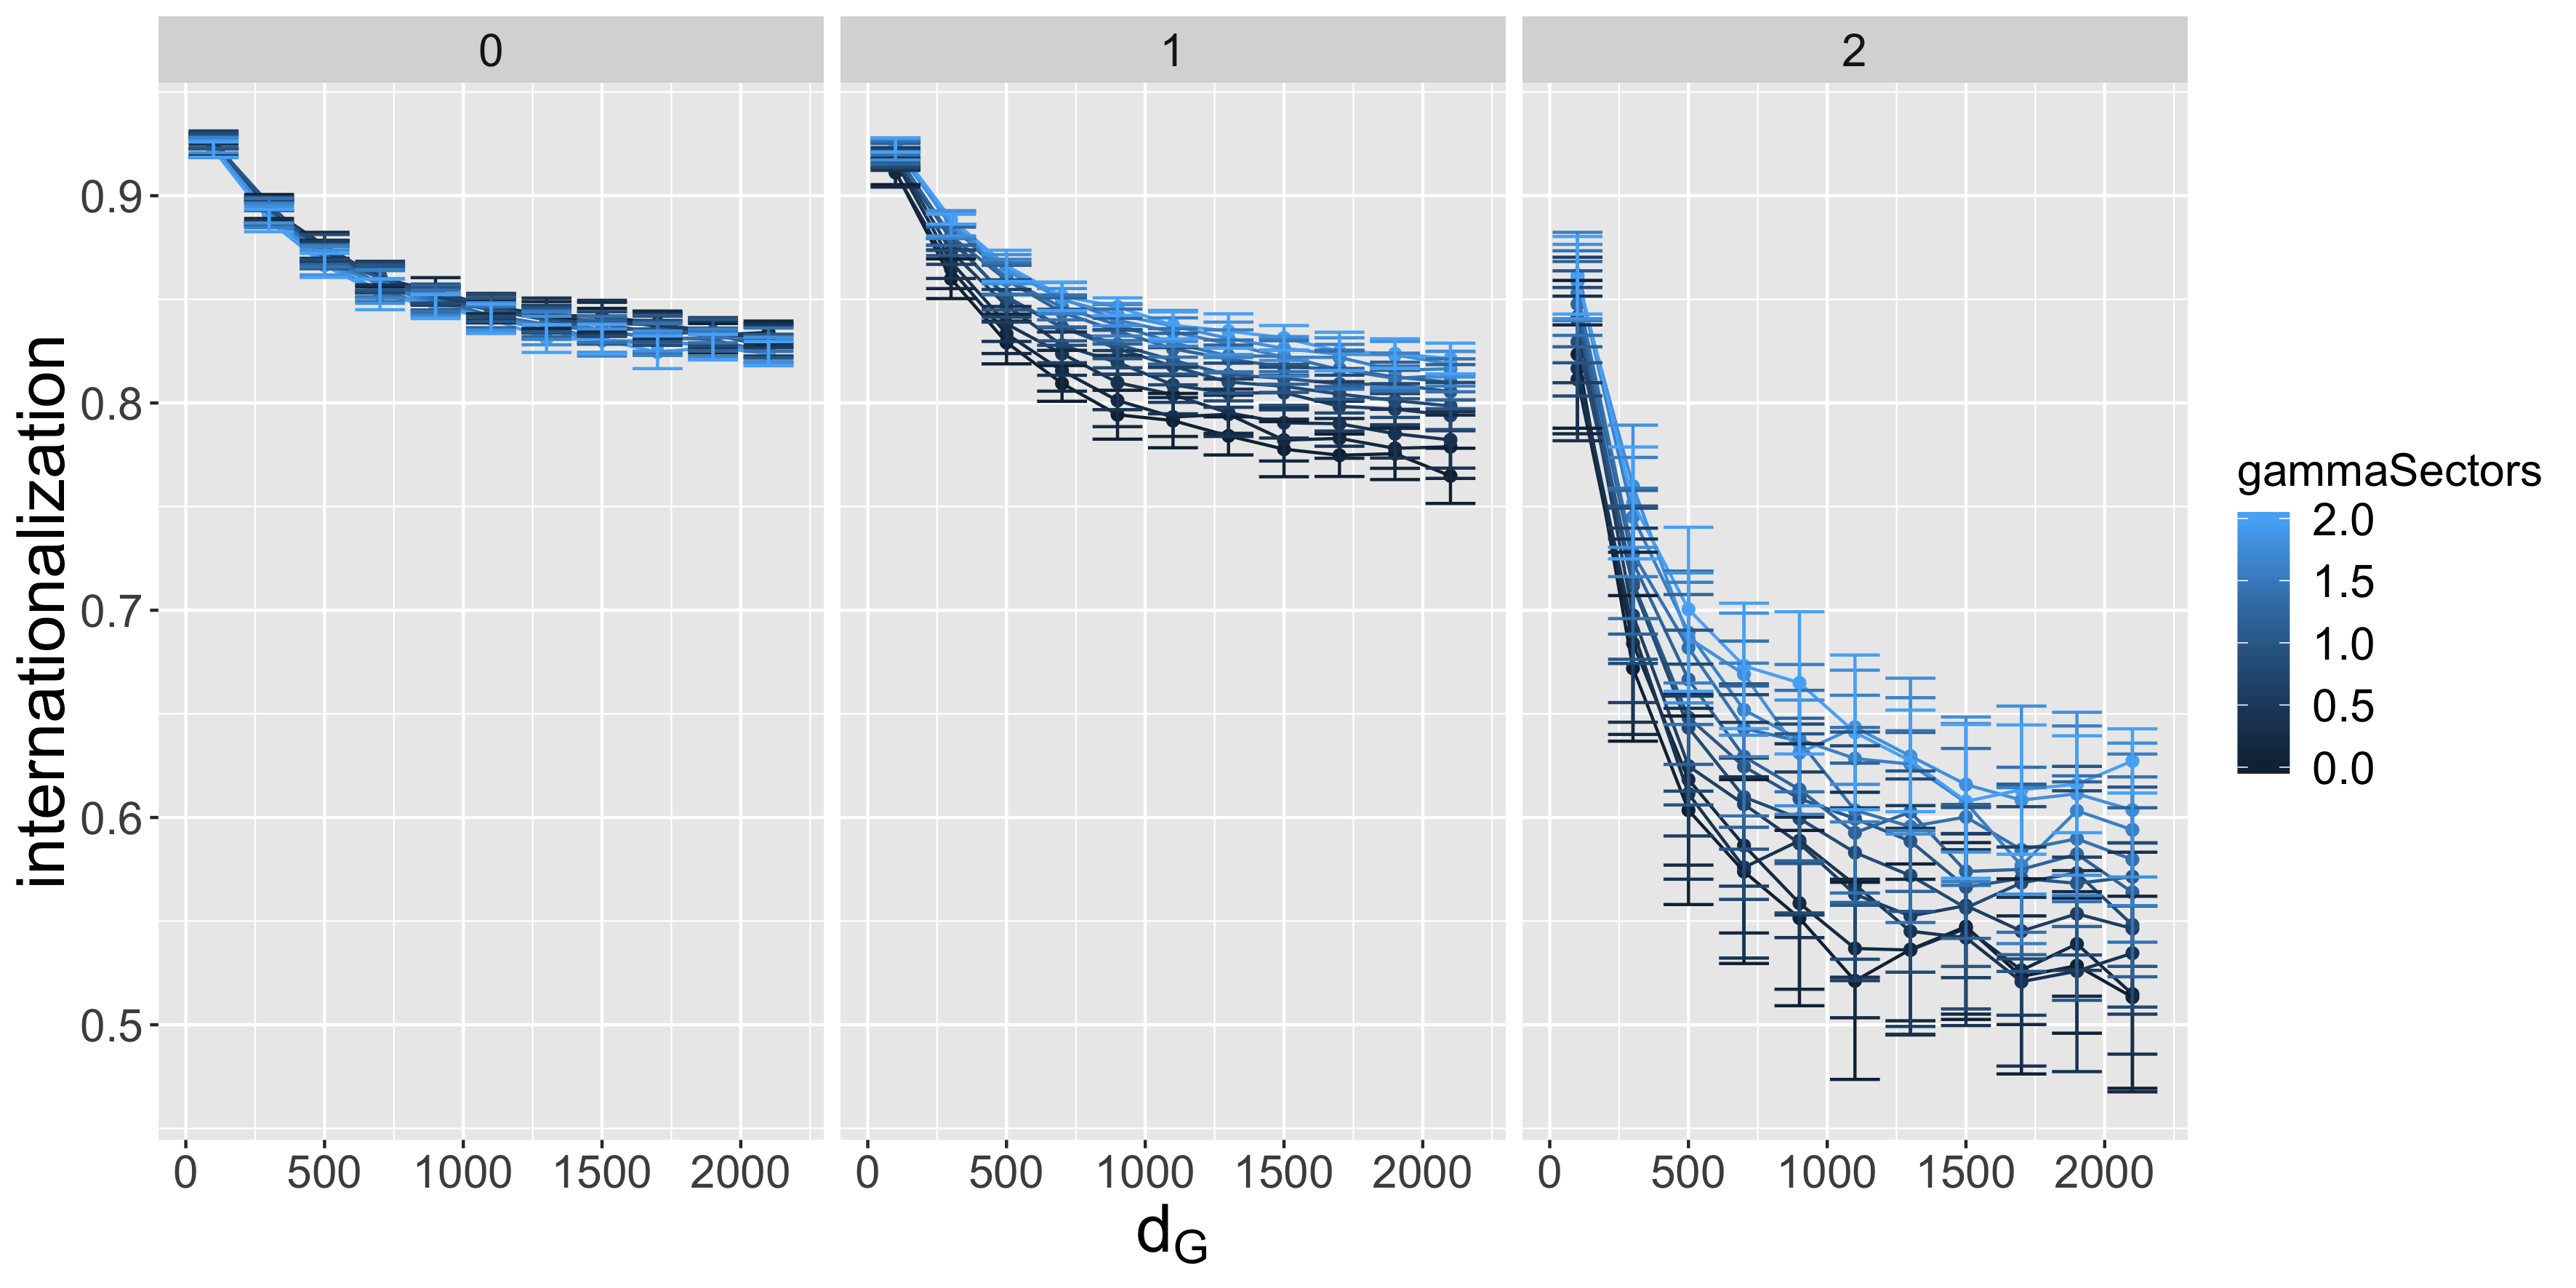
\includegraphics[width=\textwidth]{figures/internationalization_countryGravityDecay200_gammaDestination0_facetwrapgammaOrigin_colorgammaSectors.png}
    \caption{The transition as a function of interaction range depends on the influence of origin size $\gamma_F$; sector proximity $\gamma_S$ plays a role only for a large influence of the origin.}
\end{figure}



\begin{figure}
    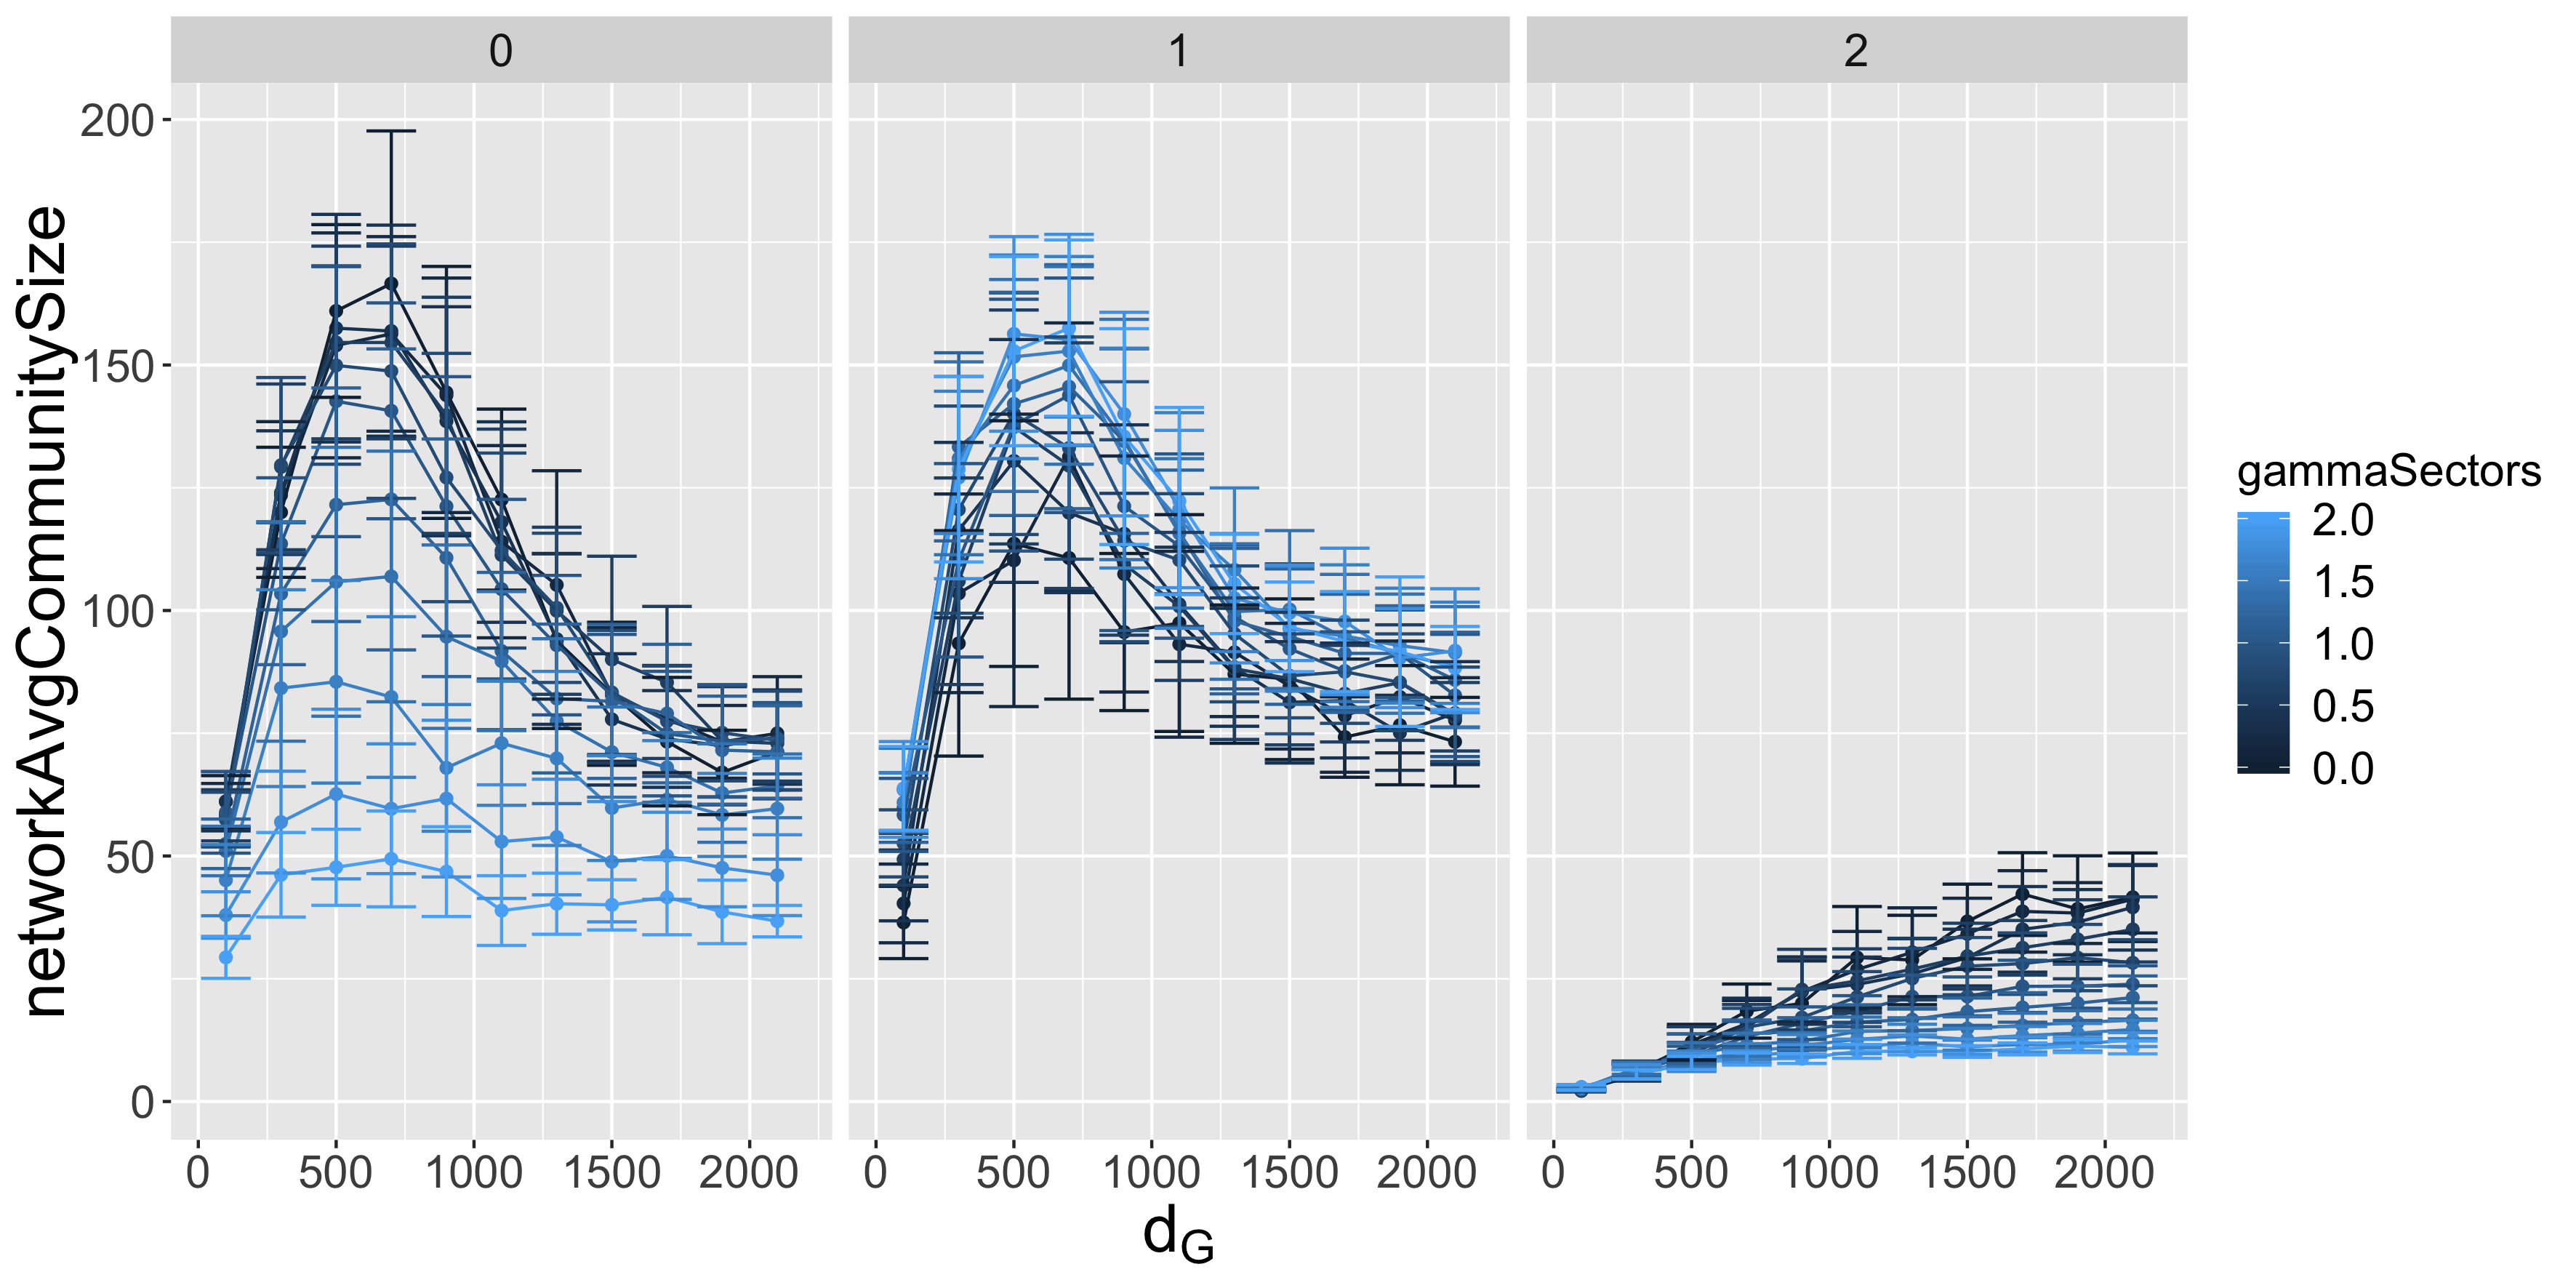
\includegraphics[height=0.6\textheight]{figures/networkAvgCommunitySize_countryGravityDecay2100_gammaDestination0_facetwrapgammaOrigin_colorgammaSectors.png}
	\caption{Maximal integration in term of community size is achieved at an intermediate value of $d_G$: emergence of a regional regime; Maximal size depends on the role of sectors $\gamma_S$, in a decreasing way when origin size is deactivated, and increasing way when $\gamma_F=1$; This regime disappear when origin size influence is too large}
\end{figure}


\subsubsection{PSE}


\subsubsection{A virtual case study: subsystem-xit}



\subsection{Real application to Europe}

% Q: do we do some "hybrid experiments"? - ex synthetic system of cities but real sector distribution




%%%%%%%%%%%%%%%
\section{Discussion}

% - evolution of city sizes (co-evolution model)

% - role of path dependency

% - towards a model with firm agents? (multi-scale ABM)



\bibliographystyle{apalike}
\bibliography{biblio}

\end{document}
